%%%%%%%%%%%%%%%%%%%%%%%%%%%%%%%%%%%%%%%%%
% Beamer Presentation
% LaTeX Template
% Version 1.0 (10/11/12)
%
% This template has been downloaded from:
% http://www.LaTeXTemplates.com
%
% License:
% CC BY-NC-SA 3.0 (http://creativecommons.org/licenses/by-nc-sa/3.0/)
%
%%%%%%%%%%%%%%%%%%%%%%%%%%%%%%%%%%%%%%%%%

%----------------------------------------------------------------------------------------
%	PACKAGES AND THEMES
%----------------------------------------------------------------------------------------

\documentclass{beamer}

\mode<presentation> {

% The Beamer class comes with a number of default slide themes
% which change the colors and layouts of slides. Below this is a list
% of all the themes, uncomment each in turn to see what they look like.

%\usetheme{default}
%\usetheme{AnnArbor}
%\usetheme{Antibes}
%\usetheme{Bergen}
%\usetheme{Berkeley}
%\usetheme{Berlin}
%\usetheme{Boadilla}
%\usetheme{CambridgeUS}
%\usetheme{Copenhagen}
%\usetheme{Darmstadt}
%\usetheme{Dresden}
%\usetheme{Frankfurt}
%\usetheme{Goettingen}
%\usetheme{Hannover}
%\usetheme{Ilmenau}
%\usetheme{JuanLesPins}
%\usetheme{Luebeck}
\usetheme{Madrid}
%\usetheme{Malmoe}
%\usetheme{Marburg}
%\usetheme{Montpellier}
%\usetheme{PaloAlto}
%\usetheme{Pittsburgh}
%\usetheme{Rochester}
%\usetheme{Singapore}
%\usetheme{Szeged}
%\usetheme{Warsaw}

% As well as themes, the Beamer class has a number of color themes
% for any slide theme. Uncomment each of these in turn to see how it
% changes the colors of your current slide theme.

%\usecolortheme{albatross}
%\usecolortheme{beaver}
%\usecolortheme{beetle}
%\usecolortheme{crane}
%\usecolortheme{dolphin}
%\usecolortheme{dove}
%\usecolortheme{fly}
%\usecolortheme{lily}
%\usecolortheme{orchid}
%\usecolortheme{rose}
%\usecolortheme{seagull}
%\usecolortheme{seahorse}
%\usecolortheme{whale}
%\usecolortheme{wolverine}

%\setbeamertemplate{footline} % To remove the footer line in all slides uncomment this line
%\setbeamertemplate{footline}[page number] % To replace the footer line in all slides with a simple slide count uncomment this line

%\setbeamertemplate{navigation symbols}{} % To remove the navigation symbols from the bottom of all slides uncomment this line
}

\usepackage{graphicx} % Allows including images
\usepackage{booktabs} % Allows the use of \toprule, \midrule and \bottomrule in tables

%----------------------------------------------------------------------------------------
%	TITLE PAGE
%----------------------------------------------------------------------------------------

\title[Stocks Project]{CS4911 Sprint 1 Presentation} % The short title appears at the bottom of every slide, the full title is only on the title page

\author{Alex Bettadapur\and Charles  Wang\and Andy Hull\and Jason Provenzano\and Kendall Merritt} % Your name
%\institute[UCLA] % Your institution as it will appear on the bottom of every slide, may be shorthand to save space
%{
%University of California \\ % Your institution for the title page
%\medskip
%\textit{john@smith.com} % Your email address
%}
%\date{\today} % Date, can be changed to a custom date

\begin{document}

\begin{frame}
\titlepage % Print the title page as the first slide
\end{frame}

\begin{frame}
\frametitle{Overview} % Table of contents slide, comment this block out to remove it
\tableofcontents % Throughout your presentation, if you choose to use \section{} and \subsection{} commands, these will automatically be printed on this slide as an overview of your presentation
\end{frame}

%----------------------------------------------------------------------------------------
%	PRESENTATION SLIDES
%----------------------------------------------------------------------------------------

%------------------------------------------------
\section{Introduction} % Sections can be created in order to organize your presentation into discrete blocks, all sections and subsections are automatically printed in the table of contents as an overview of the talk
%------------------------------------------------

%\subsection{Subsection Example} % A subsection can be created just before a set of slides with a common theme to further break down your presentation into chunks

\begin{frame}
\frametitle{Brief Introduction}
\begin{itemize}
\item Team Members
\begin{itemize}
\item Alex Bettadapur
\item Andy Hull
\item Charles Wang
\item Jason Provenzano
\item Kendall Merritt
\end{itemize}
\item Client: Everette Egun
\end{itemize}
\end{frame}

%------------------------------------------------

\section{Product Vision}
\begin{frame}
\frametitle{Product Context}
Our client wants a product to perform stock analysis to assist in trading. Currently, the client performs the analysis manually, which is a time-consuming and error-prone task. \vspace{0.3cm}

In order to make the client's task easier and more accurate, a data acquisition and analysis tool is desired.


\end{frame}

\begin{frame}
\frametitle{Deliverable}
We will deliver an application that will collect and analyze stock data based on the client's attributes on a weekly (or otherwise scheduled) basis, generate a report, and email this report to the client. \vspace{0.3cm}

Furthermore, we will create tools for the client to use independently of these scheduled reports to monitor stocks more closely.
\end{frame}

\begin{frame}
\frametitle{Initial Requirements}
The client wants to filter stocks by the following (basic) attributes: 
\begin{itemize}
\item Float: Amount of tradeable shares
\item Growth: Revenue Growth 
\item Movement: Price Movement
\end{itemize} 
and more complicated attributes as time allows. \vspace{0.3cm}

The client will receive scheduled emails containing reports listing the stocks which meet the client's thresholds.  The client also wants tools to monitor other aspects of stocks. These will be developed as time permits.
\end{frame}

\section{Design Alternatives}
\begin{frame}
\frametitle{Design Alternatives}

Since our application is intended more as a data analysis tool, the bulk of our work will be implementing these tools and thus our design does not need to be very complex. \vspace{0.3cm}

We think the main design decision is where the application should do its work. Thus we came up with the following alternatives:
\begin{itemize}
\item Native Client
\item Web Application
\item Web Server with Thin Client
\end{itemize}
\end{frame}

\begin{frame}
\frametitle{Alternative: Native Client}
We would provide the user with an application that would run on their machine. 

\begin{itemize}
\item All work is performed on the client's own machine
\item Persistent data needed by the application would be stored on the system
\item The application would have a GUI to allow the user to interact with the software to change the parameters for analysis and presentation.
\end{itemize}
\end{frame}

\begin{frame}
\frametitle{Native Client: pros and cons}
Pros
\begin{itemize}
\item Convenient; always accessible even without internet
\item The user can be given the code to maintain/develop
\item The user does not need to pay for any server/data storage services
\end{itemize}
Cons
\begin{itemize}
\item Requires user's resources
\item Platform dependent
\item User's system tied up 
\item Installation
\end{itemize}
\end{frame}

\begin{frame}
\frametitle{Alternative: Web Application}
We would provide a web service run on a server that would host a webpage where the user could interact with the software. This has the benefit of externalizing all the services so the user's own system is not needed for any part of the software. 
\begin{itemize}
\item All work is performed by a server independent of client's machine
\item Persistent data needed by the application would be stored in a database 
\item A server would host a webpage to act as a UI
\end{itemize}
\end{frame}

\begin{frame}
\frametitle{Web Application: pros and cons}
Pros
\begin{itemize}
\item Does not consume user's resources (space or computation time)
\item Platform independent
\item Can run completely independently of the user's system
\item No installation required on the user's end
\end{itemize}
Cons
\begin{itemize}
\item User may need to pay for external services
\item Internet access required to interact with application
\end{itemize}
\end{frame}

\begin{frame}
\frametitle{Alternative: Server with Thin Client}
We would provide the user with a lightweight client backed by a server. The data would be stored on the server and any computations would be performed on the server. The user would interact with the application via a small UI on their system.
\begin{itemize}
\item Most work is performed on a server, but small tasks may be run on client's machine
\item Persistent data needed by the application would be stored in a databse 
\item A small client is installed on the user's system to interact with the server
\end{itemize}
\end{frame}

\begin{frame}
\frametitle{Server with Thin Client: pros and cons}
Pros
\begin{itemize}
\item Consumes very few resources on user's system
\item (Mostly) platform independent
\item Heavy work can run independently of user's system
\item Tasks can be moved to user's system to run without internet access
\item Minimal installation required
\end{itemize}
Cons
\begin{itemize}
\item User may need to pay for external services
\item Internet access required for most tasks
\item Need to develop a client independent of the server
\end{itemize}
\end{frame}

\section{Final Design}
\begin{frame}
\frametitle{Final Design - Rationale}
We decided to implement the project as a web service. 
\begin{itemize}
\item platform independent
\item does not requiring the user's resources
\item no installation 
\end{itemize}
These considerations helped us to eliminate the native client alternative. \vspace{.3cm}

The thin client alternative was very similar to the web service alternative. However
\begin{itemize}
\item not enough functionality could be moved to the user's system 
\item extra development cost to implement 
\end{itemize}
so we decided to eliminate the thin client alternative as well
\end{frame}

\subsection{Static Design}

\begin{frame}
\frametitle{Static Design}
\begin{figure}[h!]
  \centering
  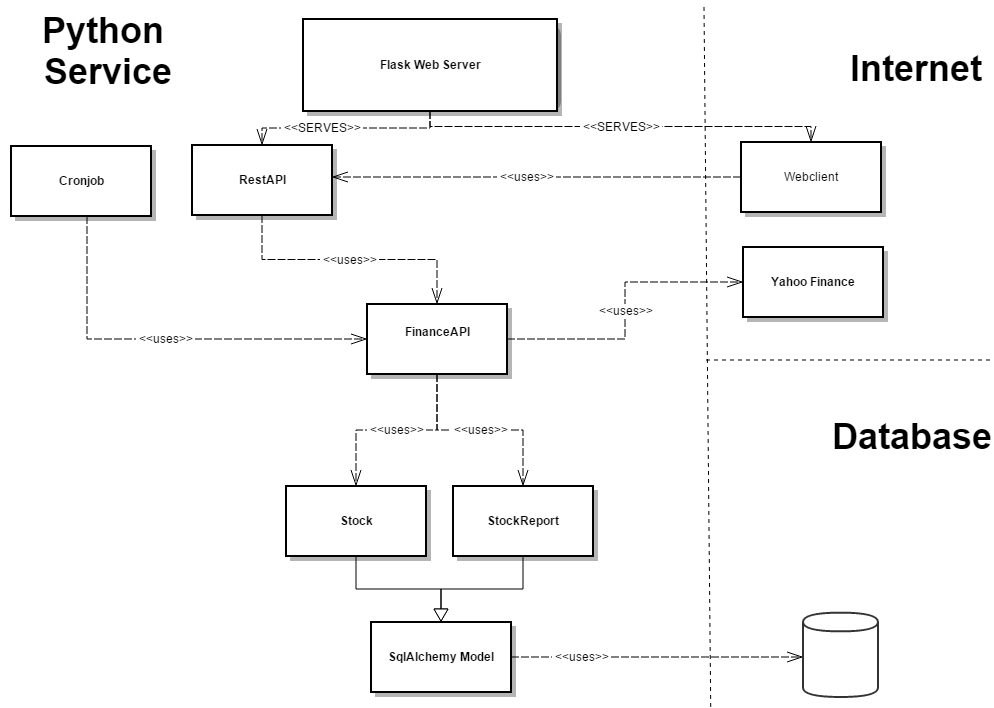
\includegraphics[scale=0.3]{stock_uml.png}
\end{figure}
\end{frame}

\begin{frame}
\frametitle{Static Design Components}
\begin{itemize}
\item webserver: This component knows how to process and fulfill requests from the web client 
\item cronjob: This component holds information about when to generate the scheduled reports
\item restAPI: This component details how to interact with the webclient
\item financeAPI: This component details how to fulfill requests by analyzing the data
\item yahoo finance API: This component provides stock information necessary to process the user's requests
\end{itemize}
\end{frame}


\begin{frame}
\frametitle{Static Design Components}
\begin{itemize}
\item webclient: This component provides a UI for the user to interact with the web server through a layer of abstraction
\item stock: This component models the stock object for the system to provide a uniform data retrieval/storage for stocks
\item stockreport: This component holds the directions for creating the stock reports that the user requested
\item sqlalchemy: This component converts stock information into database entires
\item database: This component stores all the persistent information we need about stocks to perform the user's jobs
\end{itemize}
\end{frame}

\subsection{Dynamic Design}

\begin{frame}
\frametitle{Dynamic Design}

\begin{figure}[h!]
  \centering
  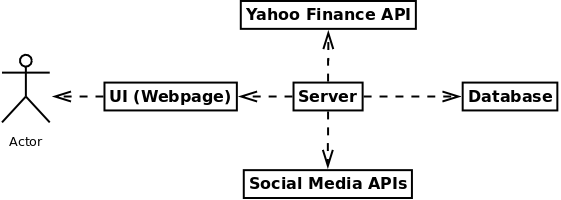
\includegraphics[scale=0.4]{UML_block.png}
\end{figure}
Essentially, the dynamic behavior of our application is that the user will interact with the UI (webpage) to request some service. The server will then fulfill this request by gathering the relevant data and reporting the results as appropriate (for example, either delivering a schedule report, or changing the state of a display on the UI).
\end{frame}

\section{Project plan}
\begin{frame}
\frametitle{Sprint 1 Burndown}
\begin{figure}[h!]
  \centering
  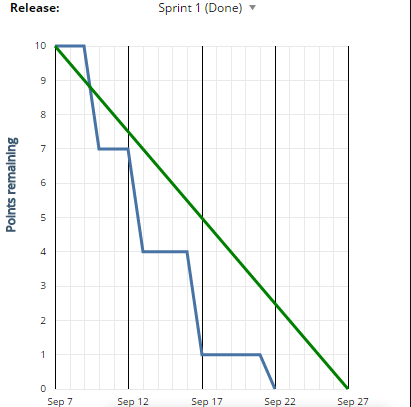
\includegraphics[scale=0.5]{burndown.png}
\end{figure}
\end{frame}

\begin{frame}
\frametitle{Pivotal Tracker}
\begin{figure}[h!]
  \centering
  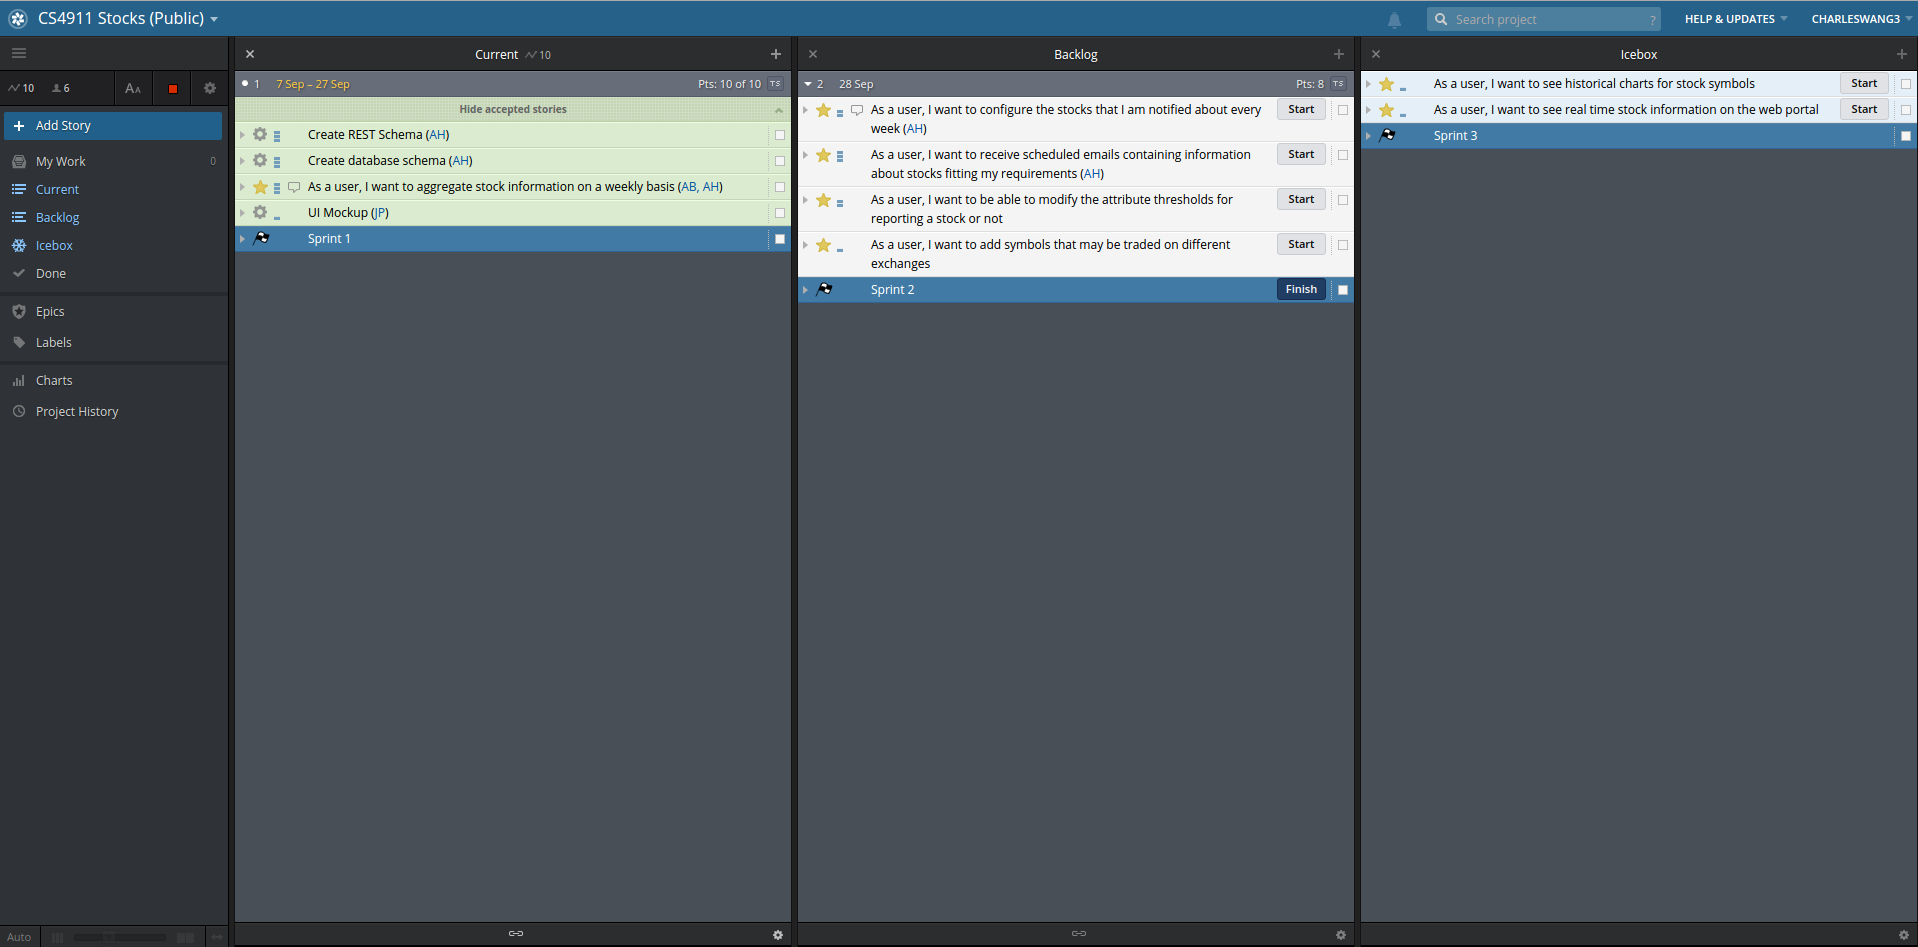
\includegraphics[scale=0.18]{PT.png}
\end{figure}
\end{frame}

\section{Status}
\begin{frame}
\frametitle{Status}
Currently, we have finished implementing the client's basic requirements (scheduled report generation based on basic attributes).
\vspace{0.3cm}

At this point, we plan to:
\begin{itemize}
\item Work on UI (webpage)
\item Work with the client to develop more complex attributes
\item Work with client to find what tools they want or need
\end{itemize}
\end{frame}

\section{Short Demo}
\begin{frame}
\frametitle{Demo}
Short Demo!
\end{frame}

\end{document}


%---------------------------------EXAMPLES BELOW
\begin{frame}
\frametitle{Bullet Points}
\begin{itemize}
\item Lorem ipsum dolor sit amet, consectetur adipiscing elit
\item Aliquam blandit faucibus nisi, sit amet dapibus enim tempus eu
\item Nulla commodo, erat quis gravida posuere, elit lacus lobortis est, quis porttitor odio mauris at libero
\item Nam cursus est eget velit posuere pellentesque
\item Vestibulum faucibus velit a augue condimentum quis convallis nulla gravida
\end{itemize}
\end{frame}

%------------------------------------------------

\begin{frame}
\frametitle{Blocks of Highlighted Text}
\begin{block}{Block 1}
Lorem ipsum dolor sit amet, consectetur adipiscing elit. Integer lectus nisl, ultricies in feugiat rutrum, porttitor sit amet augue. Aliquam ut tortor mauris. Sed volutpat ante purus, quis accumsan dolor.
\end{block}

\begin{block}{Block 2}
Pellentesque sed tellus purus. Class aptent taciti sociosqu ad litora torquent per conubia nostra, per inceptos himenaeos. Vestibulum quis magna at risus dictum tempor eu vitae velit.
\end{block}

\begin{block}{Block 3}
Suspendisse tincidunt sagittis gravida. Curabitur condimentum, enim sed venenatis rutrum, ipsum neque consectetur orci, sed blandit justo nisi ac lacus.
\end{block}
\end{frame}

%------------------------------------------------

\begin{frame}
\frametitle{Multiple Columns}
\begin{columns}[c] % The "c" option specifies centered vertical alignment while the "t" option is used for top vertical alignment

\column{.45\textwidth} % Left column and width
\textbf{Heading}
\begin{enumerate}
\item Statement
\item Explanation
\item Example
\end{enumerate}

\column{.5\textwidth} % Right column and width
Lorem ipsum dolor sit amet, consectetur adipiscing elit. Integer lectus nisl, ultricies in feugiat rutrum, porttitor sit amet augue. Aliquam ut tortor mauris. Sed volutpat ante purus, quis accumsan dolor.

\end{columns}
\end{frame}

%------------------------------------------------
\section{Second Section}
%------------------------------------------------

\begin{frame}
\frametitle{Table}
\begin{table}
\begin{tabular}{l l l}
\toprule
\textbf{Treatments} & \textbf{Response 1} & \textbf{Response 2}\\
\midrule
Treatment 1 & 0.0003262 & 0.562 \\
Treatment 2 & 0.0015681 & 0.910 \\
Treatment 3 & 0.0009271 & 0.296 \\
\bottomrule
\end{tabular}
\caption{Table caption}
\end{table}
\end{frame}

%------------------------------------------------

\begin{frame}
\frametitle{Theorem}
\begin{theorem}[Mass--energy equivalence]
$E = mc^2$
\end{theorem}
\end{frame}

%------------------------------------------------

\begin{frame}[fragile] % Need to use the fragile option when verbatim is used in the slide
\frametitle{Verbatim}
\begin{example}[Theorem Slide Code]
\begin{verbatim}
\begin{frame}
\frametitle{Theorem}
\begin{theorem}[Mass--energy equivalence]
$E = mc^2$
\end{theorem}
\end{frame}\end{verbatim}
\end{example}
\end{frame}

%------------------------------------------------

\begin{frame}
\frametitle{Figure}
Uncomment the code on this slide to include your own image from the same directory as the template .TeX file.
%\begin{figure}
%\includegraphics[width=0.8\linewidth]{test}
%\end{figure}
\end{frame}

%------------------------------------------------

\begin{frame}[fragile] % Need to use the fragile option when verbatim is used in the slide
\frametitle{Citation}
An example of the \verb|\cite| command to cite within the presentation:\\~

This statement requires citation \cite{p1}.
\end{frame}

%------------------------------------------------

\begin{frame}
\frametitle{References}
\footnotesize{
\begin{thebibliography}{99} % Beamer does not support BibTeX so references must be inserted manually as below
\bibitem[Smith, 2012]{p1} John Smith (2012)
\newblock Title of the publication
\newblock \emph{Journal Name} 12(3), 45 -- 678.
\end{thebibliography}
}
\end{frame}

%------------------------------------------------

\begin{frame}
\Huge{\centerline{The End}}
\end{frame}

%----------------------------------------------------------------------------------------

\end{document} 

Each team has 15-20 minutes for midterm (Sprint 1),
30 mins for Sprint 2 demo/design review, 30-35
minutes for final presentations
Principle purpose of midterm is project description,
design alternatives and status, and Sprint 1 demo.

Introduction of team

Team name, customer, faculty advisor, team members, their
roles
Product to be delivered (Vision)


Customer background, product context, tangible product to be
developed
Overview of requirements
Design Alternatives, Design Selected, Rationale (Solution
Approach)
Project plan (backlogs/burndown)


Project Backlog / burndown
Iteration 1 Backlog / burndown
Status (Backlogs/burndown)
Sprint 1 Demo (Demo)